% Figure: the ontology (T-Box) declared in ontology/vi-dbpedia.ttl.
\documentclass[tikz, border=4mm]{standalone}
% Shared style for the project figures. Compile each figure with XeLaTeX.
% Notation follows the IE650 Knowledge Graphs slides (University of Mannheim):
%   resource (IRI) = ellipse, literal = rectangle, labelled arrow = property,
%   unlabelled arrow = rdfs:subClassOf ("convention for this course").
\usepackage{fontspec}
% TeX Gyre Heros/Cursor: Helvetica/Courier clones with Vietnamese letters.
\setmainfont{texgyreheros}[
  Extension=.otf, UprightFont=*-regular, BoldFont=*-bold,
  ItalicFont=*-italic, BoldItalicFont=*-bolditalic]
\setmonofont{texgyrecursor}[
  Extension=.otf, UprightFont=*-regular, BoldFont=*-bold,
  ItalicFont=*-italic, BoldItalicFont=*-bolditalic]
\renewcommand{\familydefault}{\sfdefault}
\usetikzlibrary{arrows.meta, calc, fit, positioning, backgrounds,
  shapes.geometric, shapes.misc}

\definecolor{kgfill}{HTML}{FCD5B0}     % node fill used in the lecture slides
\definecolor{kgline}{HTML}{8C8C8C}
\definecolor{kgnavy}{HTML}{0B2D50}     % arrows and dbo:/W3C property labels
\definecolor{kgnew}{HTML}{C0392B}      % new terms of this project (vio:)
\definecolor{kgextfill}{HTML}{D9E8F6}  % resources of other datasets (5th star)
\definecolor{kgext}{HTML}{2E75B6}
\definecolor{kgbox}{HTML}{F4F6F8}
\definecolor{kgmuted}{HTML}{5F6B76}

\tikzset{
  every picture/.style={line join=round},
  res/.style={ellipse, draw=kgline, fill=kgfill, font=\ttfamily,
    inner xsep=1pt, inner ysep=2pt, minimum height=9.5mm},
  cls/.style={res},
  lit/.style={rectangle, draw=kgline, fill=kgfill, font=\ttfamily,
    inner xsep=5pt, minimum height=8.5mm},
  ext/.style={res, draw=kgext, fill=kgextfill},
  rel/.style={-{Stealth[length=3mm, width=2.4mm]}, draw=kgnavy, line width=1pt},
  sub/.style={rel},
  nodomain/.style={rel, dash pattern=on 4.5pt off 2.5pt},
  lbl/.style={font=\ttfamily, text=kgnavy, fill=white, inner sep=1.2pt},
  newlbl/.style={lbl, text=kgnew},
  note/.style={font=\small, text=kgmuted, align=left},
  panel/.style={draw=kgline, fill=kgbox, rounded corners=2pt, inner sep=6pt},
  heading/.style={font=\bfseries, text=kgnavy, anchor=north west},
}

\begin{document}
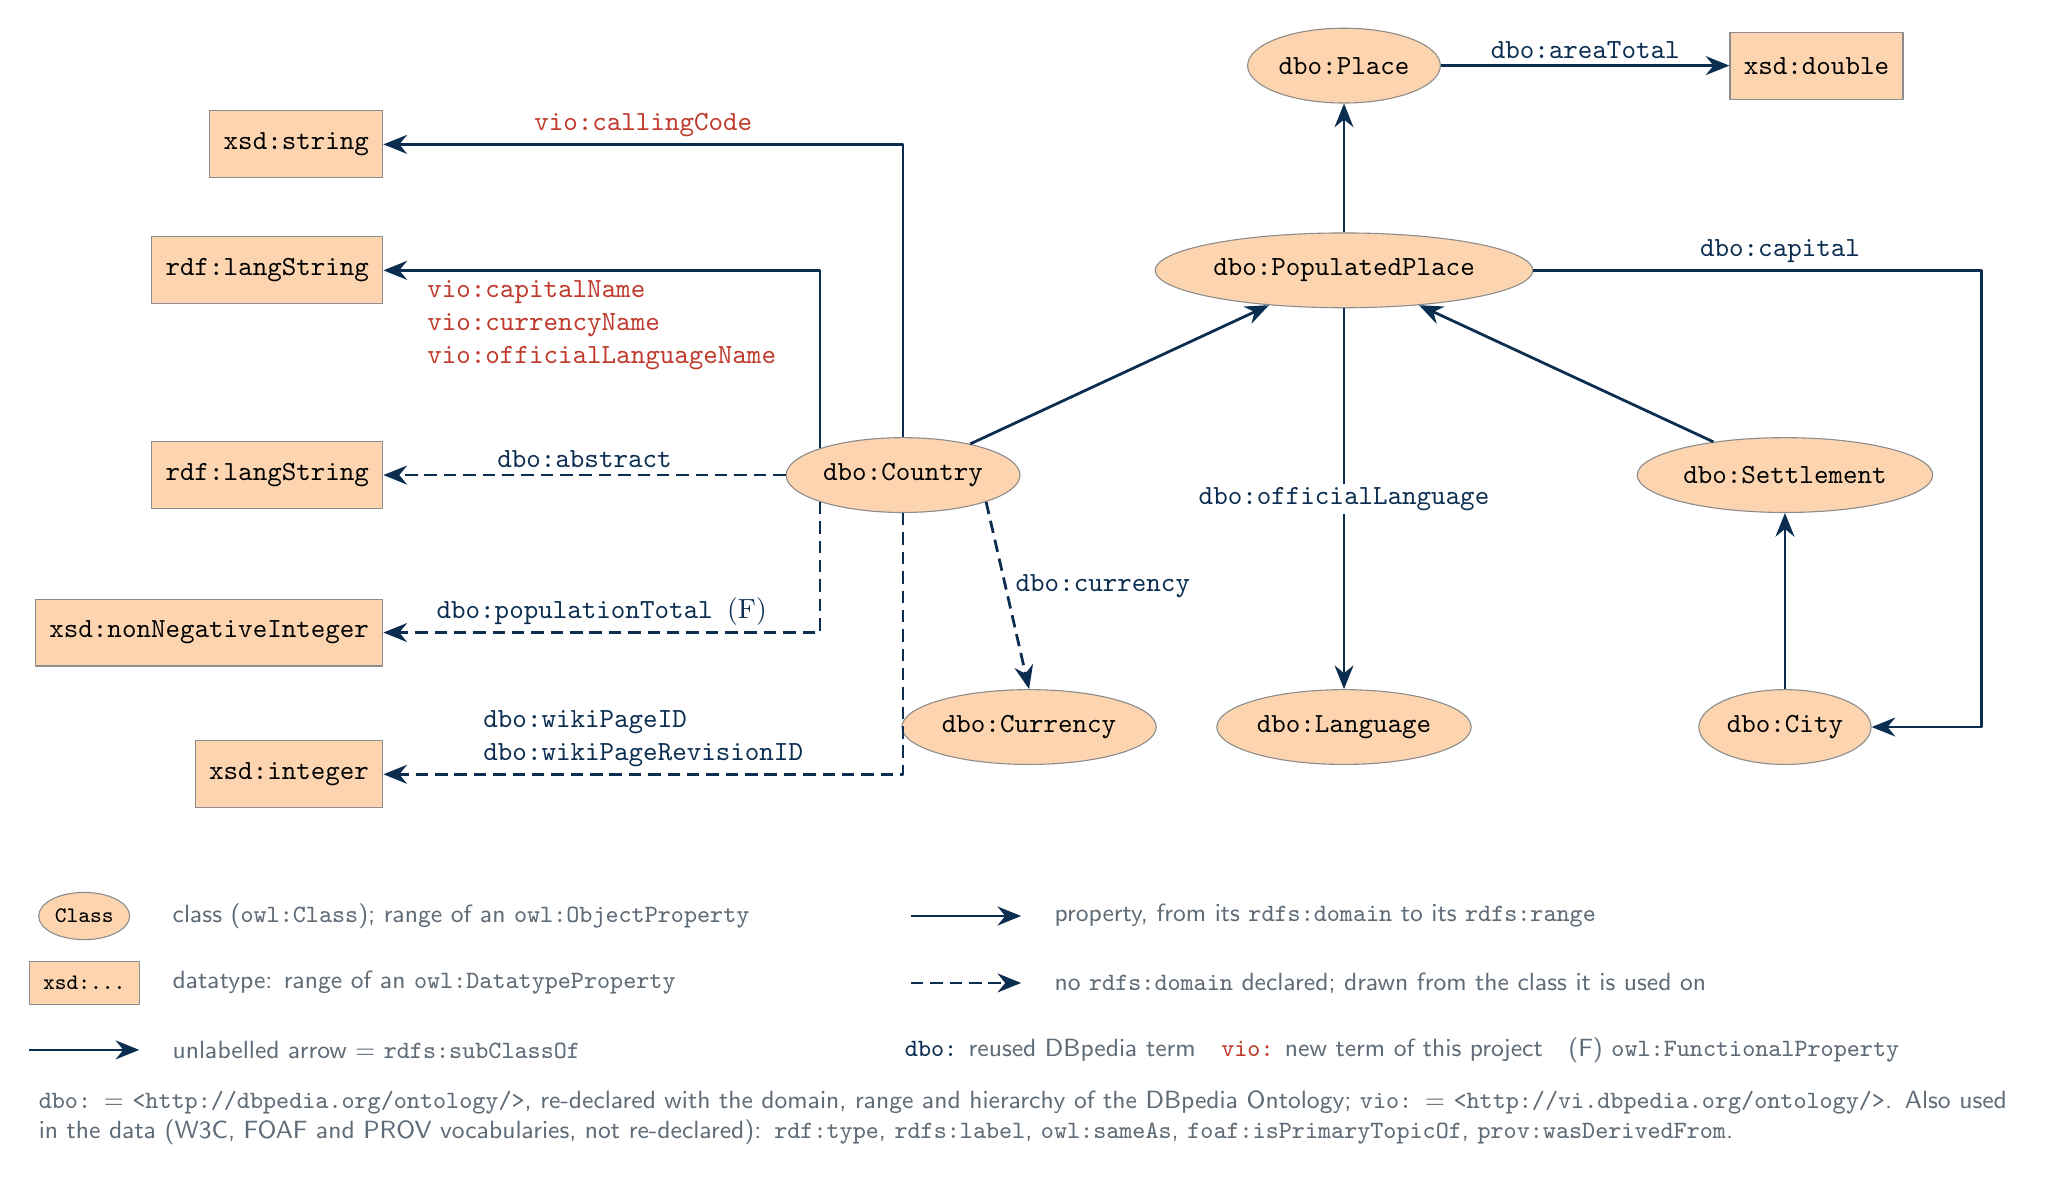
\begin{tikzpicture}

% ---- Classes and their DBpedia hierarchy (unlabelled arrow = rdfs:subClassOf)
\node[cls] (place)   at (2.6, 9.6)  {dbo:Place};
\node[cls] (pop)     at (2.6, 7.0)  {dbo:PopulatedPlace};
\node[cls] (country) at (-3.0, 4.4) {dbo:Country};
\node[cls] (settle)  at (8.2, 4.4)  {dbo:Settlement};
\node[cls] (city)    at (8.2, 1.2)  {dbo:City};
\node[cls] (lang)    at (2.6, 1.2)  {dbo:Language};
\node[cls] (cur)     at (-1.4, 1.2) {dbo:Currency};

\draw[sub] (pop) -- (place);
\draw[sub] (country) -- (pop);
\draw[sub] (settle) -- (pop);
\draw[sub] (city) -- (settle);

% ---- Object properties, from rdfs:domain to rdfs:range
\draw[rel] (pop.south) -- node[lbl, pos=0.5] {dbo:officialLanguage} (lang.north);
\draw[rel] (pop.east) -- node[lbl, above=1pt, pos=0.55] {dbo:capital} (10.7, 7.0)
  |- (city.east);
\draw[nodomain] (country.south east) -- node[lbl, right=2pt, pos=0.45] {dbo:currency} (cur.north);

% ---- Datatype properties; the range is an XML Schema / RDF datatype
\node[lit] (double) at (8.6, 9.6) {xsd:double};
\draw[rel] (place.east) -- node[lbl, above=1pt] {dbo:areaTotal} (double.west);

\node[lit, anchor=east] (str)   at (-9.6, 8.6) {xsd:string};
\node[lit, anchor=east] (names) at (-9.6, 7.0) {rdf:langString};
\node[lit, anchor=east] (abs)   at (-9.6, 4.4) {rdf:langString};
\node[lit, anchor=east] (count) at (-9.6, 2.4) {xsd:nonNegativeInteger};
\node[lit, anchor=east] (int)   at (-9.6, 0.6) {xsd:integer};

% Domain dbo:Country (new vio: terms)
\draw[rel] (country.north) |- node[newlbl, above=1pt, pos=0.75] {vio:callingCode} (str.east);
\draw[rel] (country.north west) |- node[newlbl, below=2pt, pos=0.75, align=left]
  {vio:capitalName\\vio:currencyName\\vio:officialLanguageName} (names.east);
% No rdfs:domain in the DBpedia Ontology: drawn from dbo:Country, where they are used
\draw[nodomain] (country.west) -- node[lbl, above=1pt, pos=0.5] {dbo:abstract} (abs.east);
\draw[nodomain] (country.south west) |- node[lbl, above=1pt, pos=0.75]
  {dbo:populationTotal \textrm{(F)}} (count.east);
\draw[nodomain] (country.south) |- node[lbl, above=1pt, pos=0.75, align=left]
  {dbo:wikiPageID\\dbo:wikiPageRevisionID} (int.east);

% ---- Legend
\begin{scope}[shift={(-14.3, -1.2)}]
  \node[cls, minimum height=6mm, font=\ttfamily\footnotesize] at (0.9, 0) {Class};
  \node[note, anchor=west] at (1.9, 0) {class (\texttt{owl:Class}); range of an \texttt{owl:ObjectProperty}};
  \node[lit, minimum height=5.5mm, font=\ttfamily\footnotesize] at (0.9, -0.85) {xsd:…};
  \node[note, anchor=west] at (1.9, -0.85) {datatype: range of an \texttt{owl:DatatypeProperty}};
  \draw[sub] (0.2, -1.7) -- (1.6, -1.7);
  \node[note, anchor=west] at (1.9, -1.7) {unlabelled arrow = \texttt{rdfs:subClassOf}};

  \draw[rel] (11.4, 0) -- (12.8, 0);
  \node[note, anchor=west] at (13.1, 0)
    {property, from its \texttt{rdfs:domain} to its \texttt{rdfs:range}};
  \draw[nodomain] (11.4, -0.85) -- (12.8, -0.85);
  \node[note, anchor=west] at (13.1, -0.85)
    {no \texttt{rdfs:domain} declared; drawn from the class it is used on};
  \node[note, anchor=west] at (11.2, -1.7) {\textcolor{kgnavy}{\texttt{dbo:}} reused DBpedia term\quad
    \textcolor{kgnew}{\texttt{vio:}} new term of this project\quad
    (F) \texttt{owl:FunctionalProperty}};
\end{scope}
\node[note, anchor=north west, text width=25.2cm] at (-14.1, -3.3) {%
  \texttt{dbo:} = \texttt{<http://dbpedia.org/ontology/>}, re-declared with the domain, range and
  hierarchy of the DBpedia Ontology;
  \texttt{vio:} = \texttt{<http://vi.dbpedia.org/ontology/>}.
  Also used in the data (W3C, FOAF and PROV vocabularies, not re-declared):
  \texttt{rdf:type}, \texttt{rdfs:label}, \texttt{owl:sameAs}, \texttt{foaf:isPrimaryTopicOf},
  \texttt{prov:wasDerivedFrom}.};

\end{tikzpicture}
\end{document}
